\chapter{Implementacija i korisničko sučelje}
		
		
		\section{Korištene tehnologije i alati}
		
			Komunikacija u timu realizirana je putem mobilne aplikacije  \underline{WhatsApp}\footnote{\url{https://www.whatsapp.com}}. 
			Za izradu UML dijagrama korišten je alat \underline{Astah Professional}\footnote{\url{https://astah.net/products/astah-professional/}}, a kao sustav za upravljanje izvornim kodom \underline{Git}\footnote{\url{https://git-scm.com/}}. 
			Udaljeni repozitorij projekta je dostupan na web platformi \underline{GitLab}\footnote{\url{https://gitlab.com/}}.
			\par
			Kao razvojno okruženje korišten je \underline{Eclipse}\footnote{\url{https://www.eclipse.org/}} - integrirano razvojno okruženje. Eclipse je većinom pisan u Javi i prvenstveno se koristi za razvoj Java aplikacija, ali koristi se i za razvoj aplikacija u drugim programskim jezicima kao što su C, C++, PHP, Python i još mnogi drugi.
			\par
			Za razvoj korisničkog sučelja i frontenda korišten je uređivač teksta \underline{VSCode}\footnote{\url{https://code.visualstudio.com/}}. Taj uređivač teksta je danas jedan od najrasprostranjenijih i koristi se u svim sferama industrije. 
			\par
			Aplikacija je napisana u \underline{Javi}\footnote{\url{https://www.java.com/en/}} koristeći ekosustav \underline{Java Spring}\footnote{\url{https://spring.io/}} za
			izradu backenda te \underline{React}\footnote{\url{https://reactjs.org/}} i \underline{JavaScript}\footnote{\url{https://www.javascript.com/}} za izradu frontenda. 
			\par
			Za bazu podataka koristili smo (\underline{PostgreSQL}\footnote{\url{https://www.postgresql.org/}}).
			
			
			\eject 
		
	
		\section{Ispitivanje programskog rješenja}
			
			\textbf{\textit{dio 2. revizije}}\\
			
			 \textit{U ovom poglavlju je potrebno opisati provedbu ispitivanja implementiranih funkcionalnosti na razini komponenti i na razini cijelog sustava s prikazom odabranih ispitnih slučajeva. Studenti trebaju ispitati temeljnu funkcionalnost i rubne uvjete.}
	
			
			\subsection{Ispitivanje komponenti}
			\textit{Potrebno je provesti ispitivanje jedinica (engl. unit testing) nad razredima koji implementiraju temeljne funkcionalnosti. Razraditi \textbf{minimalno 6 ispitnih slučajeva} u kojima će se ispitati redovni slučajevi, rubni uvjeti te izazivanje pogreške (engl. exception throwing). Poželjno je stvoriti i ispitni slučaj koji koristi funkcionalnosti koje nisu implementirane. Potrebno je priložiti izvorni kôd svih ispitnih slučajeva te prikaz rezultata izvođenja ispita u razvojnom okruženju (prolaz/pad ispita). }
			
			
			
			\subsection{Ispitivanje sustava}
			
			 \textit{Potrebno je provesti i opisati ispitivanje sustava koristeći radni okvir Selenium\footnote{\url{https://www.seleniumhq.org/}}. Razraditi \textbf{minimalno 4 ispitna slučaja} u kojima će se ispitati redovni slučajevi, rubni uvjeti te poziv funkcionalnosti koja nije implementirana/izaziva pogrešku kako bi se vidjelo na koji način sustav reagira kada nešto nije u potpunosti ostvareno. Ispitni slučaj se treba sastojati od ulaza (npr. korisničko ime i lozinka), očekivanog izlaza ili rezultata, koraka ispitivanja i dobivenog izlaza ili rezultata.\\ }
			 
			 \textit{Izradu ispitnih slučajeva pomoću radnog okvira Selenium moguće je provesti pomoću jednog od sljedeća dva alata:}
			 \begin{itemize}
			 	\item \textit{dodatak za preglednik \textbf{Selenium IDE} - snimanje korisnikovih akcija radi automatskog ponavljanja ispita	}
			 	\item \textit{\textbf{Selenium WebDriver} - podrška za pisanje ispita u jezicima Java, C\#, PHP koristeći posebno programsko sučelje.}
			 \end{itemize}
		 	\textit{Detalji o korištenju alata Selenium bit će prikazani na posebnom predavanju tijekom semestra.}
			
			\eject 
		
		
		\section{Dijagram razmještaja}
			
			Dijagrami razmještaja prikazuju topologiju sustava i odnos sklopovskih i programskih dijelova. Olakšavaju nam vizualizaciju razmještaja fizičkog dijela sustava i sklopovlja. Sustav se sastoji od korisničkog i poslužiteljskog računala. Korisnik na svojem računalu preko web preglednika pristupa aplikaciji. Korisničko računalo komunicira s poslužiteljskim računalom preko HTTP veze. Na poslužiteljskom se računalu nalaze Web poslužitelj i poslužitelj baze podataka. 
			
			\begin{figure}[H]
				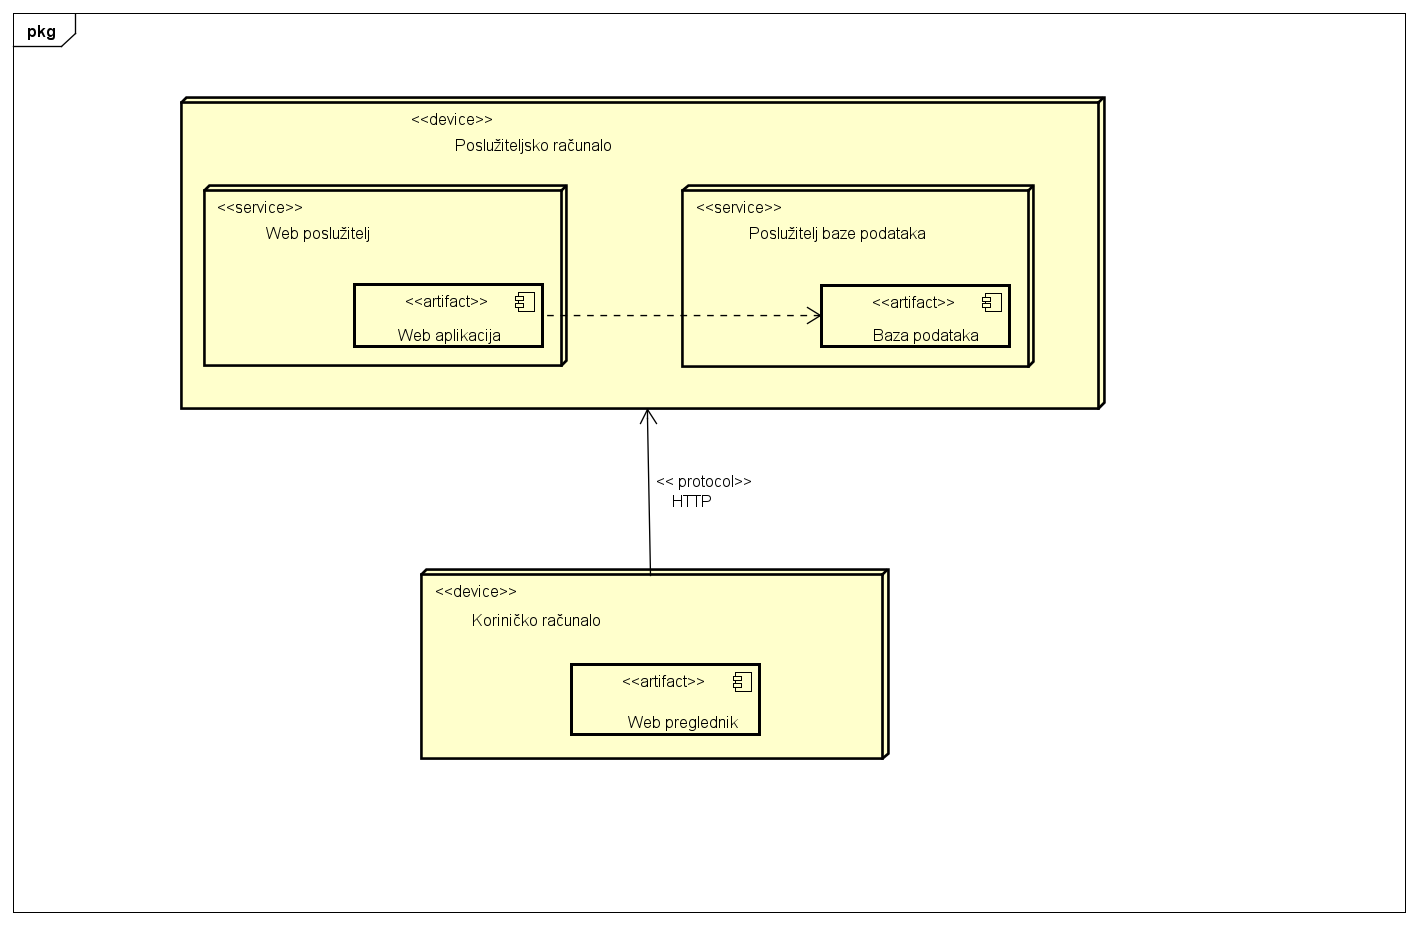
\includegraphics[width=\textwidth]{slike/Dijagram_razmjestaja.png}
				\centering
				\caption{Dijagram razmještaja}
				\label{fig:dijagram_razmjestaja}
			\end{figure}
			
			\eject 
		
		\section{Upute za puštanje u pogon}
		
			\textbf{\textit{dio 2. revizije}}\\
		
			 \textit{U ovom poglavlju potrebno je dati upute za puštanje u pogon (engl. deployment) ostvarene aplikacije. Na primjer, za web aplikacije, opisati postupak kojim se od izvornog kôda dolazi do potpuno postavljene baze podataka i poslužitelja koji odgovara na upite korisnika. Za mobilnu aplikaciju, postupak kojim se aplikacija izgradi, te postavi na neku od trgovina. Za stolnu (engl. desktop) aplikaciju, postupak kojim se aplikacija instalira na računalo. Ukoliko mobilne i stolne aplikacije komuniciraju s poslužiteljem i/ili bazom podataka, opisati i postupak njihovog postavljanja. Pri izradi uputa preporučuje se \textbf{naglasiti korake instalacije uporabom natuknica} te koristiti što je više moguće \textbf{slike ekrana} (engl. screenshots) kako bi upute bile jasne i jednostavne za slijediti.}
			
			
			 \textit{Dovršenu aplikaciju potrebno je pokrenuti na javno dostupnom poslužitelju. Studentima se preporuča korištenje neke od sljedećih besplatnih usluga: \href{https://aws.amazon.com/}{Amazon AWS}, \href{https://azure.microsoft.com/en-us/}{Microsoft Azure} ili \href{https://www.heroku.com/}{Heroku}. Mobilne aplikacije trebaju biti objavljene na F-Droid, Google Play ili Amazon App trgovini.}
			
			
			\eject 